\section{SORA 3 Payload Design}
\label{sec:Design}

\subsection{Payload Structure}
One major design goal of the SORA 3 mission was to make the overall layout of the payload more modular such that each subsystem was not dependent on the presence of other subsystems.
This was a major change from previous missions in which systems and components were not organized leading to massive disorganization across the payload.
The modular structure not only organized the systems, but it made it such that the now independent systems could function in the absence of other systems, thus leading to continued functionality of the payload in the event of an in situ failure.

The modular organization was accomplished by compartmentalizing each subsystem into its own structure.
The payload was broken up into four main substructures: the astrobiology system, the two radiation containers, and the electronics box.
The electronics box served to join all systems together, and the other subsystems could easily be added or removed to the electronics box.
The electronics box was made from an easy-to-form PVC/acrylic, which has been proven to work well for previous missions as it can withstand the extreme environment of the stratosphere and is easily machinable.
The construction and materials of the astrobiology box and the radiation containers are discussed in their respective sections.

% Include image of the payload layout
% Talk about physical construction and layout of the payload

\begin{figure}[h!]
	\begin{center}
		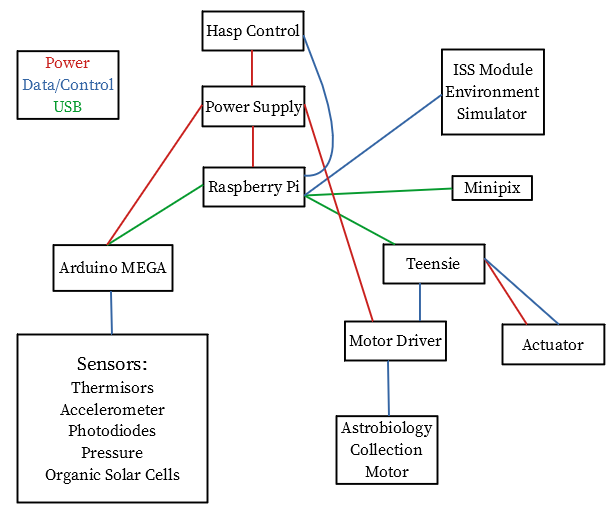
\includegraphics[width=0.75\textwidth]{figures/sys_overview.png}
		\caption{An overview of the payload's electronics configuration.}
		\label{fig:sys_overview}
	\end{center}
\end{figure}
% Talk about the hardware (PSU, RPi, etc.)
\subsection{Hardware and Electronics}
\subsubsection{Power Supply}

The SORA 3 payload used a WinSystems PPM-DC-ATX-P power supply unit (PSU).
This unit has several properties that are very attractive for applications such as this. 
To power the flight computer and hardware we received the \SI{30}{\volt} DC supply from HASP which we fed to our PSU that supplied our flight computer and sensor electronics with \SI{+5}{\volt}, and our current-to-voltage operational amplifiers with \SI{+12}{\volt} and \SI{-12}{\volt}.
The pins used for the SORA 3 payload are marked in Figure \ref{fig:psu-outputs}.
It has an input range of \SIrange{10}{50}{\volt}, so the PSU is capable of withstanding any variation in voltage caused by HASP's depleting batteries.
Additionally, this PSU is rated to operate from \SIrange{-40}{85}{\celsius}, which is within the environmental variation of temperatures in the stratosphere.
More technical details can be found on its datasheet at Ref. \cite{WinSystems-PSU}.

\begin{figure}[h!]
	\begin{center}
		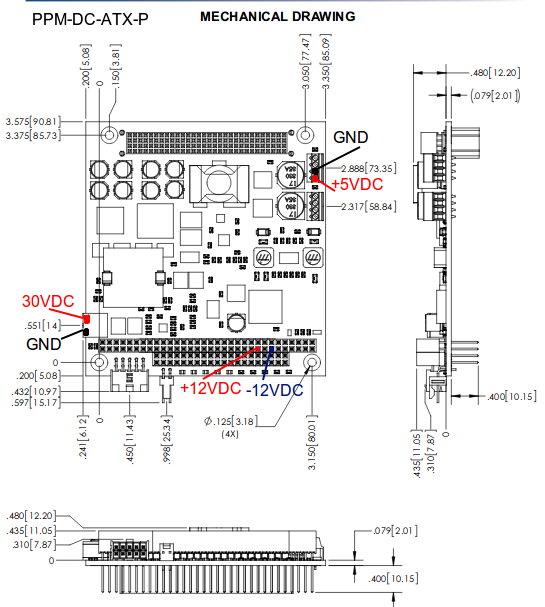
\includegraphics[width=0.75\textwidth]{figures/psu-pins.png}
		\caption{A detailed schematic of the PSU taken from its datasheet. The pins that were used for the SORA 3 payload are marked on the diagram.}
		\label{fig:psu-outputs}
	\end{center}
\end{figure}

\subsubsection{Flight Computer}
A Raspberry Pi was chosen as the main component of the flight computer as we needed a platform that was capable of storing an SQL database for the large volume of data we had planned to catalogue from the solar cells. An SQL database was found to be necessary due to the serial down-link limit imposed by HASP. We also opted to utilize an Arduino MEGA in order to control the majority of the sensors such as the thermistors for temperature readings, multiple photodiodes for capturing light intensity at the solar cells, a pressure sensor for monitoring altitude, and the array of current-to-voltage converters for characterizing the solar cells. Additionally, the Arduino MEGA sent control signals to an Arduino Nano, a very small footprint microcontroller, which controlled an actuator and a DC stepper motor that were required to operate the mechanical system to facilitate the Astrobiology experiment.


\subsubsection{DC Stepper Motor}
The AccelStepper Arduino Library developed by AirSpayce \cite{AccelStepper} was integral to the functionality of our motor.
In the initial stages of programming the astrobiology robotic components, issues arose when we discovered the stepper motor would miscount the number of steps it had taken while accelerating, due to the fact that we had programmed it to jump from a velocity of zero to a high velocity without any initial acceleration, resulting steps being missed in the hardware of the motor and therefore an overshoot on the counted steps versus how many the motor actually took.
This was problematic because our motor needed to be returned to a specific location to be retracted into the box, due to our rectangular design.
If the motor was off the mark, the payload would be damaged when the lid retracted.
In order to accomplish this goal, we needed to specify in our code exactly how many steps to take to turn back to this position.

Setting the acceleration of the motor within the regular stepper motor library was not an option with the initial setup.
While there is a function that accomplished this, it blocks the rest of the code from running until the motor has finished its turn.
This was not ideal because it meant that our sensor network would be unable to collect data during the time the motor took to spin. The AccelStepper library solved this issue.
Based on speed profiles for these types of motors developed by David Austin in "Generate stepper-motor speed profiles in real time", the AccelStepper library allows the appropriate speed to be calculated in real-time, preventing the hang up in the code. 

We chose a stepper motor as the motor for our astrobiology collection system due to its ability to rotate \SI{360}{\degree} degrees continuously.
We rejected a simpler servo motor for this reason - most only have the ability to turn \SI{180}{\degree} and then return to their original position.
To accomplish our goal of continuous \SI{360}{\degree} rotation, stepper motors were lightweight, inexpensive, and dependable enough to accomplish this task effectively.
We chose the NEMA 14 model due to its ability to provide the correct amount of torque needed for our project, while also being able to support the appropriate amount of weight.
A DRV8834 motor driver was used to control the voltage supplied to the motor, which made it possible to easily control to torque supplied by the motor.
The motor circuit is shown in Figure \ref{fig:motor-circuit}.
% Our actuator was chosen due to its compact size and dependability. 

\begin{figure}[h!]
	\begin{center}
		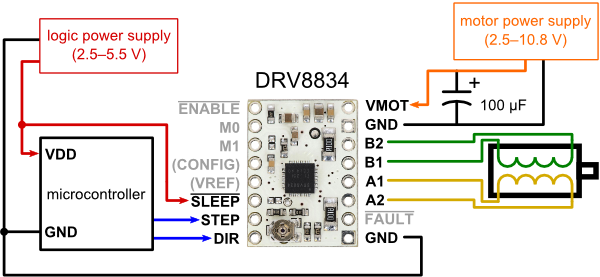
\includegraphics[width=0.75\textwidth]{figures/stepper-motor-circuit.png}
		\caption{Circuit showing the stepper motor with its driver. The motor power supply was a direct connection to the PSU, and the logic power supply was provided by the Arduino Nano.}
		\label{fig:motor-circuit}
	\end{center}
\end{figure}
